\subsection{Polohové vztahy přímek v rovině}
\label{subsec:Positional_relations_lines_plane}

Dosud jsme se zabývali především popisem jedné přímky. Nyní budeme
uvažovat dvě přímky v téže rovině a určovat jejich vzájemnou polohu.

Při řešení budeme využívat údaje, které jednotlivé tvary rovnic
poskytují: směrové vektory, normálové vektory a směrnice. V případě
různoběžných přímek budeme také určovat jejich průsečík.

\subsubsection{Možné vzájemné polohy dvou přímek}
\label{subsubsec:Possible_relative_positions_lines}

Dvě přímky v rovině mohou být \textbf{různoběžné},
\textbf{rovnoběžné} nebo \textbf{totožné}. Mimoběžné přímky,
které nemají společný bod a zároveň nejsou rovnoběžné, se mohou
vyskytovat až v prostoru.

\begin{definition}\label{def:Intersecting_lines_plane}
    Dvě přímky v rovině nazýváme \textbf{různoběžnými}, jestliže mají
    právě jeden společný bod, který nazýváme jejich
    \textbf{průsečíkem}.
\end{definition}

\begin{definition}\label{def:Parallel_lines_plane}
    Dvě různé přímky v rovině nazýváme \textbf{rovnoběžnými}, jestliže
    mají stejný směr a nemají žádný společný bod.
\end{definition}

\begin{definition}\label{def:Coincident_lines_plane}
    Dvě přímky v rovině nazýváme \textbf{totožnými}, jestliže mají
    všechny body společné, a představují tedy tutéž množinu bodů.
\end{definition}

Jednotlivé možné vzájemné polohy dvou přímek v rovině jsou znázorněny
na obrázku \ref{fig:Relative_positions_lines_plane}.

\begin{figure}[H]
    \centering

    % -------------------------------------------------
    % Různoběžné přímky
    % -------------------------------------------------
    \begin{minipage}{0.32\textwidth}
        \centering
        \begin{tikzpicture}[scale=0.9]

            \coordinate (P) at (0,0);

            \draw[thin, <->] (-2,-1.2) -- (2,1.2)
                node[above right] {$p$};

            \draw[thin, <->] (-1.8,1.5) -- (1.8,-1.5)
                node[below right] {$q$};

            \fill (P) circle (2pt)
                node[below] {$P$};

            \draw[vector] (0.5,0.3) -- (1.5,0.91) node[midway, above, sloped]{$\vec{u}_p$};
            \draw[vector] (-0.5,0.4) -- (-1.2,1) node[midway, above, sloped] {$\vec{u}_q$};

        \end{tikzpicture}

        \small různoběžné
    \end{minipage}
    \hfill
    % -------------------------------------------------
    % Rovnoběžné přímky
    % -------------------------------------------------
    \begin{minipage}{0.32\textwidth}
        \centering
        \begin{tikzpicture}[scale=0.9]

            \draw[thin, <->] (-2,0.7) -- (2,0.7)
                node[above right] {$p$};

            \draw[thin, <->] (-2,-0.7) -- (2,-0.7)
                node[above right] {$q$};

            \draw[vector] (0.5,0.7) -- (1.2,0.7) node[midway, above, sloped]{$\vec{u}_p$};
            \draw[vector] (0.2,-0.7) -- (-1,-0.7) node[midway, above, sloped] {$\vec{u}_q$};

        \end{tikzpicture}

        \small rovnoběžné
    \end{minipage}
    \hfill
    % -------------------------------------------------
    % Totožné přímky
    % -------------------------------------------------
    \begin{minipage}{0.32\textwidth}
        \centering
        \begin{tikzpicture}[scale=0.9]

            \draw[thin, <->] (-2,0) -- (2,0);
            \node[below right] at (1.2,0) {$p = q$};

            \draw[vector] (-0.5,0) -- (-1.75,0) node[midway, above, sloped]{$\vec{u}_p$};
            \draw[vector] (1,0) -- (1.7,0) node[midway, above, sloped] {$\vec{u}_q$};

        \end{tikzpicture}

        \small totožné
    \end{minipage}

    \caption{Možné vzájemné polohy dvou přímek v rovině.}
    \label{fig:Relative_positions_lines_plane}
\end{figure}

\subsubsection{Vzájemná poloha parametricky zadaných přímek}
\label{subsubsec:Relative_position_parametric_lines}

U parametrického vyjádření je směr přímky určen jejím směrovým
vektorem. Vzájemnou polohu dvou parametricky zadaných přímek proto
budeme určovat především porovnáním jejich směrových vektorů.

Uvažujme přímky $p$ a $q$ zadané parametricky ve tvaru
\begin{align}
    p: X &= A+t\vec{u},
    \qquad t\in\mathbb{R},
    \label{eq:Parametric_line_p_relative_position}\\
    q: X &= B+s\vec{v},
    \qquad s\in\mathbb{R},
    \label{eq:Parametric_line_q_relative_position}
\end{align}
kde $A$ a $B$ jsou zvolené body jednotlivých přímek a $\vec{u}$,
$\vec{v}$ jsou jejich nenulové směrové vektory.

Pro každou přímku používáme jiný parametr, v našem případě $t$ a $s$,
protože hodnota parametru určuje, o jaký násobek příslušného směrového
vektoru se ze zvoleného bodu posuneme. Hodnota parametru potřebná
k dosažení společného bodu z bodu $A$ proto obecně nemusí být stejná
jako hodnota parametru potřebná k dosažení téhož bodu z bodu $B$.

Vzájemnou polohu přímek určíme nejprve porovnáním jejich směrových
vektorů.

Jestliže směrové vektory $\vec{u}$ a $\vec{v}$ nejsou rovnoběžné,
tedy neexistuje číslo $k\in\mathbb{R}$, pro které by platilo
\[
    \vec{v}=k\vec{u},
\]
mají přímky různé směry. Protože obě přímky leží v jedné rovině,
protínají se právě v jednom bodě a jsou tedy různoběžné podle definice \ref{def:Intersecting_lines_plane}.

Jestliže naopak existuje číslo
$k\in\mathbb{R}\setminus\{0\}$ takové, že
\[
    \vec{v}=k\vec{u},
\]
mají přímky stejný směr. V takovém případě jsou přímky buď rovnoběžné,
nebo totožné, a proto musíme ještě ověřit, zda jeden zvolený bod jedné
přímky leží také na přímce druhé.

Pokud zvolený bod $B$ přímky $q$ neleží na přímce $p$,
nemají přímky žádný společný bod a jsou proto rovnoběžné podle definice \ref{def:Parallel_lines_plane}. 
Jestliže naopak bod $B$ na přímce $p$ leží, mají obě přímky
společný bod a zároveň stejný směr, takže jsou totožné podle definice \ref{def:Coincident_lines_plane}.

Celý rozhodovací postup můžeme shrnout následovně:
\[
\begin{array}{c|c}
\text{Podmínka}
&
\text{Vzájemná poloha přímek}
\\
\hline
\vec{u}\text{ a }\vec{v}\text{ nejsou rovnoběžné}
&
\text{přímky jsou různoběžné}
\\[1mm]
\vec{v}=k\vec{u},\ k\neq0,\ \text{a }B\notin p
&
\text{přímky jsou rovnoběžné}
\\[1mm]
\vec{v}=k\vec{u},\ k\neq0,\ \text{a }B\in p
&
\text{přímky jsou totožné}
\end{array}
\]
Rozhodovací postup můžeme také shrnout pomocí schématu na obrázku
\ref{fig:Relative_position_parametric_lines_decision}.

\begin{remark}\label{rem:Alternative_test_coincident_lines}
    Místo přímého dosazování bodu $B$ do parametrického vyjádření
    přímky $p$ můžeme určit vektor
    \[
        \overrightarrow{AB}=B-A.
    \]
    Bod $B$ leží na přímce $p$ právě tehdy, když existuje číslo
    $\lambda\in\mathbb{R}$ takové, že
    \[
        \overrightarrow{AB}=\lambda\vec{u}.
    \]
    Tato podmínka zahrnuje také případ $A=B$, pro který je
    $\lambda=0$.

    Jsou-li současně směrové vektory obou přímek rovnoběžné, jsou
    přímky totožné. Dosazování bodu do parametrického vyjádření však
    zároveň procvičuje postup potřebný při hledání průsečíku, a proto
    jej budeme v následujících příkladech používat častěji.
\end{remark}

\begin{figure}[H]
    \centering
    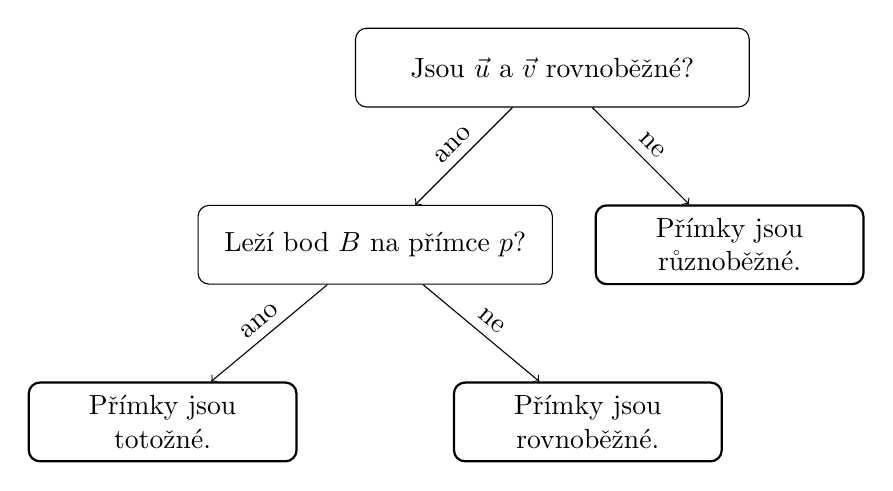
\begin{tikzpicture}[scale=0.9, every node/.style={align=center}]

        % Uzly
        \node[draw, rounded corners, minimum width=5cm, minimum height=1cm]
            (start) at (0,0)
            {Jsou $\vec{u}$ a $\vec{v}$ rovnoběžné?};

        \node[draw, rounded corners, minimum width=4.5cm, minimum height=1cm]
            (point) at (-2.5,-2.5)
            {Leží bod $B$ na přímce $p$?};

        \node[draw, rounded corners, minimum width=3.4cm, minimum height=1cm, thick]
            (intersecting) at (2.5,-2.5)
            {Přímky jsou\\různoběžné.};

        \node[draw, rounded corners, minimum width=3.4cm, minimum height=1cm, thick]
            (coincident) at (-5.5,-5)
            {Přímky jsou\\totožné.};

        \node[draw, rounded corners, minimum width=3.4cm, minimum height=1cm, thick]
            (parallel) at (0.5,-5)
            {Přímky jsou\\rovnoběžné.};

        % Šipky
        \draw[->] (start) -- (point)
            node[midway, above, sloped] {ano};

        \draw[->] (start) -- (intersecting)
            node[midway, above, sloped] {ne};

        \draw[->] (point) -- (coincident)
            node[midway, above, sloped] {ano};

        \draw[->] (point) -- (parallel)
            node[midway, above, sloped] {ne};

    \end{tikzpicture}
    \caption{Postup při určování vzájemné polohy parametricky zadaných přímek v rovině.}
    \label{fig:Relative_position_parametric_lines_decision}
\end{figure}

\paragraph{Rovnoběžné přímky}

Jak již bylo řečeno, jsou-li směrové vektory dvou přímek navzájem rovnoběžné, nemůžeme pouze
z této skutečnosti rozhodnout, zda jsou přímky rovnoběžné, nebo totožné.
Musíme ještě ověřit, zda jeden zvolený bod jedné přímky leží také na
druhé přímce.

\begin{example}\label{exa:Parallel_parametric_lines}
    Určete vzájemnou polohu přímek $p$ a $q$ zadaných bodem
    a směrovým vektorem:
    \[
        p:\ A[-1;3],\qquad \vec{u}=(-1;2),
    \]
    \[
        q:\ B[1;1],\qquad \vec{v}=(2;-4).
    \]

    Nejprve zjistíme, zda jsou směrové vektory $\vec{u}$ a $\vec{v}$
    navzájem rovnoběžné. Hledáme tedy číslo $k\in\mathbb{R}$, pro které
    platí
    \[
        \vec{v}=k\vec{u}.
    \]

    Po dosazení souřadnic dostáváme
    \[
        (2;-4)=k(-1;2).
    \]
    Z jednotlivých souřadnic vyplývá
    \begin{align*}
        2 &= -k \Rightarrow  k=-2,\\
        -4 &= 2k \Rightarrow k=-2.
    \end{align*}

    Z obou souřadnic vyšla stejná hodnota $k=-2$, a proto jsou směrové
    vektory rovnoběžné. Přímky $p$ a $q$ jsou tedy buď rovnoběžné,
    nebo totožné.

    Nyní ověříme, zda bod $A[-1;3]$ leží na přímce $q$. Parametrické
    vyjádření přímky $q$ je
    \begin{align*}
        q: x &= 1+2s,\\
           y &= 1-4s;
           \quad s\in\mathbb{R}.
    \end{align*}

    Dosadíme souřadnice bodu $A[-1;3]$:
    \begin{align*}
        -1 &= 1+2s,\\
        3 &= 1-4s.
    \end{align*}

    Z první rovnice získáme
    \begin{align*}
        -1 &= 1+2s,\\
        -2 &= 2s,\\
        s &= -1.
    \end{align*}
    Z druhé rovnice však vychází
    \begin{align*}
        3 &= 1-4s,\\
        2 &= -4s,\\
        s &= -\tfrac{1}{2}.
    \end{align*}

    Z rovnic vyšly různé hodnoty parametru, takže bod $A$ na přímce
    $q$ neleží. Přímky mají rovnoběžné směrové vektory, ale nemají
    společný bod, a proto jsou rovnoběžné:
    \[
        p\parallel q.
    \]
\end{example}

\paragraph{Různoběžné přímky a jejich průsečík}

Jestliže směrové vektory dvou přímek nejsou navzájem rovnoběžné, jsou
přímky v rovině různoběžné a mají právě jeden společný bod. Tento bod
nazýváme \textbf{průsečíkem přímek}.

Průsečík musí současně ležet na obou přímkách, a jeho souřadnice proto
musí vyhovovat parametrickým rovnicím přímky $p$ i přímky $q$. Při
hledání průsečíku tedy položíme odpovídající souřadnice obou přímek
sobě rovny a vyřešíme vzniklou soustavu rovnic.

\begin{remark}\label{rem:Different_parameters_parametric_lines}
    Při porovnávání dvou parametricky vyjádřených přímek musíme pro
    každou přímku použít jiný parametr. Zápisy
    \[
        p:\ X=A+t\vec{u}
        \qquad\text{a}\qquad
        q:\ X=B+s\vec{v}
    \]
    proto používají parametry $t$ a $s$.

    Stejný bod může být totiž na první přímce získán například pro
    $t=1$, zatímco na druhé přímce může témuž bodu odpovídat hodnota
    $s=-1$. Použití stejného parametru v obou přímkách by znamenalo
    neoprávněný předpoklad, že se k průsečíku z obou zvolených bodů
    dostaneme pomocí stejného násobku rozdílných směrových vektorů.
\end{remark}

\begin{example}\label{exa:Intersecting_parametric_lines}
    Určete vzájemnou polohu přímek
    \[
        \begin{aligned}
            p:\quad x &= -1+3t,\\
                     y &= 1+t;
                     \quad t\in\mathbb{R}
        \end{aligned}
        \qquad\text{a}\qquad
        \begin{aligned}
            q:\quad x &= 1-s,\\
                     y &= -2s;
                     \quad s\in\mathbb{R}.
        \end{aligned}
    \]
    Jsou-li přímky různoběžné, určete jejich průsečík.

    Směrové vektory přímek jsou
    \[
        \vec{u}=(3;1),
        \qquad
        \vec{v}=(-1;-2).
    \]

    Nejprve ověříme, zda existuje číslo $k$, pro které platí
    \[
        \vec{v}=k\vec{u}.
    \]
    Z první souřadnice dostáváme
    \[
        -1=3k
        \qquad\Rightarrow\qquad
        k=-\frac13,
    \]
    zatímco z druhé souřadnice získáme
    \[
        -2=k.
    \]

    Hodnoty čísla $k$ se neshodují, takže směrové vektory nejsou
    rovnoběžné. Přímky $p$ a $q$ jsou proto různoběžné a mají právě
    jeden průsečík.

    Souřadnice průsečíku musí vyhovovat oběma parametrickým vyjádřením.
    Položíme proto odpovídající souřadnice sobě rovny:
    \begin{align*}
        p_x &= q_x,\\
        p_y &= q_y,
    \end{align*}
    což po dosazení parametrických rovnic přímek $p$ a $q$ dává soustavu
    \begin{align*}
        -1+3t &= 1-s,\\
        1+t &= -2s.
    \end{align*}

    Po úpravě získáme soustavu
    \begin{align*}
        3t+s &= 2,\\
        t+2s &= -1.
    \end{align*}

    Z první rovnice vyjádříme parametr $s$:
    \[
        s=2-3t.
    \]
    Dosadíme do druhé rovnice, abychom získali hodnotu parametru $t$:
    \begin{align*}
        t+2(2-3t) &= -1,\\
        t+4-6t &= -1,\\
        -5t &= -5,\\
        t &= 1.
    \end{align*}

    Hodnotu parametru $s$ dopočítáme zpětným dosazením do vztahu pro $s$:
    \[
        s=2-3\cdot1=-1.
    \]

    Souřadnice průsečíku nyní vypočítáme dosazením parametru $t=1$
    do parametrického vyjádření přímky $p$:
    \begin{align*}
        x &= -1+3\cdot1=2,\\
        y &= 1+1=2.
    \end{align*}

    Průsečíkem přímek je tedy bod
    \[
        P[2;2].
    \]

    Výsledek můžeme ověřit také dosazením hodnoty $s=-1$ do přímky $q$:
    \begin{align*}
        x &= 1-(-1)=2,\\
        y &= -2\cdot(-1)=2.
    \end{align*}

    Řešením soustavy rovnic pro parametry je dvojice
    \[
        (t;s)=(1;-1).
    \]
    Po dosazení jedné z těchto hodnot do odpovídajícího parametrického
    vyjádření jsme získali společný bod
    \[
        P[2;2].
    \]

    Průsečíkem přímek $p$ a $q$ je proto bod $P[2;2]$, což zapisujeme
    \[
        p\cap q=\{P[2;2]\}.
    \]
    
\end{example}

\begin{remark}\label{rem:Parameters_are_not_intersection_coordinates}
    Hodnoty parametrů $t$ a $s$ nejsou souřadnicemi průsečíku.
    Parametry pouze určují, jakým násobkem směrového vektoru se musíme
    posunout ze zvoleného bodu příslušné přímky. Souřadnice průsečíku
    získáme až následným dosazením vypočítané hodnoty parametru do
    parametrického vyjádření jedné z přímek.
\end{remark}

\paragraph{Totožné přímky}

Jsou-li směrové vektory dvou přímek rovnoběžné a zároveň jeden zvolený
bod první přímky leží na druhé přímce, obsahují obě přímky tentýž bod
a mají stejný směr. V takovém případě mají všechny body společné a jsou
totožné.

\begin{example}\label{exa:Coincident_parametric_lines}
    Určete vzájemnou polohu přímek
    \[
        \begin{aligned}
            p:\quad x &= -2 + 2t,\\
                    y &= 1 - t;
                    \quad t\in\mathbb{R}
        \end{aligned}
        \qquad\text{a}\qquad
        \begin{aligned}
            q:\quad x &= 4 - 4s,\\
                    y &= -2 + 2s;
                    \quad s\in\mathbb{R}.
        \end{aligned}
    \]
    Z parametrických rovnic vyčteme zvolené body a směrové vektory:
    \[
        A[-2;1],
        \qquad
        \vec{u}=(2;-1),
    \]
    \[
        B[4;-2],
        \qquad
        \vec{v}=(-4;2).
    \]

    Směrové vektory jsou rovnoběžné, protože
    \[
        \vec{v}=-2\vec{u}.
    \]

    Přímky jsou proto buď rovnoběžné, nebo totožné. 
    Ověříme, zda bod $A[-2;1]$ leží na přímce $q$. Dosadíme jeho souřadnice:
    \begin{align*}
        -2 &= 4-4s,\\
        1 &= -2+2s.
    \end{align*}

    Z první rovnice získáme
    \[
        s=\frac32,
    \]
    a z druhé rovnice rovněž
    \[
        s=\frac32.
    \]

    Bod $A$ tedy leží na přímce $q$. Přímky mají rovnoběžné směrové
    vektory a společný bod, a proto jsou totožné:
    \[
        p=q.
    \]

    Totožnost můžeme ověřit také řešením soustavy rovnic pro společné
    body:
    \begin{align*}
        -2+2t &= 4-4s,\\
        1-t &= -2+2s.
    \end{align*}

    Po úpravě první rovnice dostáváme
    \[
        t+2s=3,
    \]
    zatímco úpravou druhé rovnice získáme tutéž podmínku
    \[
        t+2s=3.
    \]

    Obě rovnice soustavy jsou tedy ekvivalentní, takže soustava má nekonečně mnoho řešení. 
    Každému bodu přímky odpovídá dvojice parametrů $t$ a $s$, která splňuje vztah
    \[
        t+2s=3.
    \]
    Protože má soustava nekonečně mnoho řešení, 
    mají přímky nekonečně mnoho společných bodů. Jejich průnikem je tedy celá přímka:
    \[
        p\cap q=p=q.
    \]
\end{example}

\paragraph{Kolmé přímky}

Kolmost je zvláštním případem různoběžnosti. Dvě parametricky zadané
přímky jsou kolmé právě tehdy, když jsou kolmé jejich směrové vektory.

Pro přímky se směrovými vektory $\vec{u}$ a $\vec{v}$ tedy platí
\[
    p\perp q
    \quad\Longleftrightarrow\quad
    \vec{u}\cdot\vec{v}=0.
\]

Protože jsou směrové vektory nenulové, nemohou být v tomto případě
rovnoběžné. Kolmé přímky se tedy v rovině protínají právě v jednom
bodě.

Určování průsečíku dvou parametricky vyjádřených přímek můžeme využít
také v geometrických úlohách. Typickým příkladem je výpočet souřadnic
paty výšky v trojúhelníku, protože pata výšky je průsečíkem přímky
obsahující jednu stranu trojúhelníku a přímky, která prochází protějším
vrcholem a je k této straně kolmá.

\begin{example}\label{exa:Foot_of_altitude_parametric_lines}
    Určete souřadnice paty výšky $v_c$ v trojúhelníku $ABC$, jehož
    vrcholy jsou
    \[
        A[-2;-1],\qquad B[6;-5],\qquad C[3;4].
    \]

    Výška $v_c$ je vedena z vrcholu $C$ kolmo ke straně $AB$.
    Její pata, kterou označíme $P_C$, proto leží současně na přímce
    obsahující stranu $AB$ i na výšce $v_c$. Bod $P_C$ tedy nalezneme
    jako průsečík těchto dvou přímek.

    Nejprve určíme směrový vektor přímky obsahující stranu $AB$:
    \[
        \overrightarrow{AB}
        =
        (6-(-2);-5-(-1))
        =
        (8;-4).
    \]

    Směrový vektor můžeme nahradit jeho jednodušším nenulovým násobkem:
    \[
        \vec{u}_{AB}=(2;-1).
    \]

    Přímka $p_{AB}$ procházející bodem $A[-2;-1]$ má tedy parametrické
    vyjádření
    \begin{align*}
        p_{AB}: x &= -2+2t,\\
                y &= -1-t;
                \quad t\in\mathbb{R}.
    \end{align*}

    Směrový vektor výšky $v_c$ musí být kolmý ke směrovému vektoru
    $\vec{u}_{AB}=(2;-1)$. Můžeme proto zvolit například vektor
    \[
        \vec{u}_{v_c}=(1;2),
    \]
    protože
    \[
        (2;-1)\cdot(1;2)=2-2=0.
    \]

    Výška $v_c$ prochází vrcholem $C[3;4]$, a proto má parametrické
    vyjádření
    \begin{align*}
        v_c: x &= 3+s,\\
             y &= 4+2s;
             \quad s\in\mathbb{R}.
    \end{align*}

    Pata výšky $P_C$ leží na obou přímkách, a proto musí její souřadnice
    vyhovovat oběma parametrickým vyjádřením. Položíme tedy odpovídající
    souřadnice sobě rovny:
    \begin{align*}
        -2+2t &= 3+s,\\
        -1-t &= 4+2s.
    \end{align*}

    Po úpravě získáme soustavu
    \begin{align*}
        2t-s &= 5,\\
        t+2s &= -5.
    \end{align*}

    Z první rovnice vyjádříme parametr $s$:
    \[
        s=2t-5.
    \]

    Dosadíme jej do druhé rovnice:
    \begin{align*}
        t+2(2t-5) &= -5,\\
        t+4t-10 &= -5,\\
        5t &= 5,\\
        t &= 1.
    \end{align*}

    Hodnotu parametru $s$ dopočítáme zpětným dosazením:
    \[
        s=2\cdot1-5=-3.
    \]

    Souřadnice paty výšky získáme například dosazením hodnoty $t=1$
    do parametrického vyjádření přímky $p_{AB}$:
    \begin{align*}
        x &= -2+2\cdot1=0,\\
        y &= -1-1=-2.
    \end{align*}

    Pata výšky $v_c$ má tedy souřadnice
    \[
        P_C[0;-2].
    \]

    Výsledek můžeme ověřit také dosazením hodnoty $s=-3$ do
    parametrického vyjádření výšky:
    \begin{align*}
        x &= 3+(-3)=0,\\
        y &= 4+2\cdot(-3)=-2.
    \end{align*}

    Obě parametrická vyjádření určují stejný bod, a proto je hledanou
    patou výšky skutečně bod
    \[
        P_C[0;-2].
    \]
\end{example}
\subsubsection{Vzájemná poloha přímek zadaných obecnými rovnicemi}
\label{subsubsec:Relative_position_general_lines}

U přímek zadaných obecnými rovnicemi můžeme jejich vzájemnou polohu
určovat pomocí normálových vektorů, které získáme přímo z koeficientů
u proměnných $x$ a $y$. V případě různoběžných přímek jejich průsečík
určíme řešením soustavy obou rovnic.

Uvažujme přímky
\[
    p:X=A+t\vec{u},
    \qquad
    q:X=B+s\vec{v},
    \qquad
    t,s\in\mathbb{R}.
\]

Uvažujme přímky
\begin{align}
    p &: a_1x+b_1y+c_1=0,
    \label{eq:General_line_p_relative_position}\\
    q &: a_2x+b_2y+c_2=0.
    \label{eq:General_line_q_relative_position}
\end{align}
Jejich normálové vektory jsou
\[
    \vec{n}_p=(a_1;b_1),
    \qquad
    \vec{n}_q=(a_2;b_2).
\]

Vzájemnou polohu přímek můžeme určit porovnáním jejich normálových
vektorů. Směrový vektor je s příslušnou přímkou rovnoběžný, zatímco
normálový vektor je k ní kolmý. Geometrický vztah mezi směrovými
a normálovými vektory obou přímek je znázorněn na obrázku
\ref{fig:Direction_normal_vectors_lines}.

Protože pootočením obou směrů o $90^\circ$ se jejich vzájemná
rovnoběžnost nezmění, platí
\[
    \vec{u}_p\parallel\vec{u}_q
    \quad\Longleftrightarrow\quad
    \vec{n}_p\parallel\vec{n}_q.
\]

Jestliže normálové vektory přímek nejsou rovnoběžné, nejsou rovnoběžné
ani jejich směrové vektory. Přímky proto mají různé směry a v rovině
se protínají právě v jednom bodě. Jsou tedy různoběžné podle definice
\ref{def:Intersecting_lines_plane}. Taková situace je znázorněna
na obrázku \ref{fig:Direction_normal_vectors_lines}.

Jestliže jsou naopak normálové vektory rovnoběžné, mají přímky stejný
směr. V takovém případě mohou být přímky buď rovnoběžné, nebo totožné.
K rozlišení těchto dvou možností již nestačí porovnat pouze koeficienty
$a_1$, $b_1$, $a_2$ a $b_2$, ale musíme porovnat všechny tři
koeficienty jejich obecných rovnic.

\begin{figure}[H]
    \centering
    \begin{tikzpicture}[scale=0.8]
       
        % Osy
        \draw[<->, thin]
            (-7,0) -- (4,0)
            node[right] {$x$};

        \draw[<->, thin]
            (0,-3) -- (0,5)
            node[above] {$y$};

        % Číselné hodnoty na ose x
        \foreach \x in {-6,-5,...,-1,1,2,...,4}
        {
            \draw (\x,0.08) -- (\x,-0.08);
            \node[below, font=\scriptsize] at (\x,0) {$\x$};
        }

        % Číselné hodnoty na ose y
        \foreach \y in {-3,-2,-1,1,2,...,4}
        {
            \draw (0.08,\y) -- (-0.08,\y);
            \node[left, font=\scriptsize] at (0,\y) {$\y$};
        }

        % Počátek soustavy
        \node[below left, font=\scriptsize] at (0,0) {$O$};

        % -------------------------------------------------
        % Přímka r_1: 2x - 3y + 6 = 0
        % tedy y = 2/3 x + 2
        % -------------------------------------------------

        \draw[thick, <->] (-6,-2) -- (3,4)
            node[pos=0.02, below right, black] {$p$};

        % -------------------------------------------------
        % Přímka r_2: x + 2y + 2 = 0
        % tedy y = -1/2 x - 1
        % -------------------------------------------------

        \draw[thick,<->] (-6,2) -- (2,-2)
            node[pos=0.02, below left, black] {$q$};

        % -------------------------------------------------
        % Směrový a normálový vektor přímky p
        % -------------------------------------------------

        % Společný počáteční bod
        \coordinate (C) at (-0.78,1.48);

        % Směrový vektor u_p
        \draw[vector] (C) -- (1.51385,3.00923)
            node[midway, below, sloped] {$\vec{u}_p$};

        % Normálový vektor n_p
        \draw[vector] (C) -- (-2.30923,3.77385)
            node[midway, right] {$\vec{n}_p$};

        % Ručně nakreslená značka pravého úhlu
        \draw (-0.558,1.628) -- (-0.706,1.850) -- (-0.928,1.702);

        % -------------------------------------------------
        % Směrový a normálový vektor přímky q
        % -------------------------------------------------

        % Společný počáteční bod
        \coordinate (F) at (-4.992,1.496);

        % Směrový vektor w
        \draw[vector] (F) -- (-3,0.5)
            node[midway, above, sloped] {$\vec{u}_q$};

        % Normálový vektor b
        \draw[vector] (F) -- (-3.996,3.488)
            node[midway, left] {$\vec{n}_q$};

        % Ručně nakreslená značka pravého úhlu
        \draw (-4.724,1.362) -- (-4.590,1.630) -- (-4.858,1.764);

    \end{tikzpicture}

    \caption{Směrové a normálové vektory různoběžných přímek $p$ a $q$.}
    \label{fig:Direction_normal_vectors_lines}
\end{figure}

Celý postup můžeme shrnout následovně:
\[
\begin{array}{c|c}
\text{Podmínka}
&
\text{Vzájemná poloha přímek}
\\
\hline
(a_2;b_2)\neq k(a_1;b_1)
&
\text{přímky jsou různoběžné}
\\[1mm]
(a_2;b_2)=k(a_1;b_1),\ (a_2;b_2;c_2)\neq k(a_1;b_1;c_1)
&
\text{přímky jsou rovnoběžné}
\\[1mm]
(a_2;b_2;c_2)=k(a_1;b_1;c_1)
&
\text{přímky jsou totožné}
\end{array}
\]
kde $k\in\mathbb{R}\setminus\{0\}$.

Prakticky můžeme rovnoběžnost normálových vektorů ověřit také pomocí vztahu,
což vychází z důlesku ze vztahu pro skalární součin (viz poznámka \ref{rem:Fast_orthogonal_vector})
\begin{equation}\label{eq:Parallel_general_lines_condition}
    a_1b_2-a_2b_1=0.
\end{equation}
Jestliže levá strana není rovna nule, normálové vektory nejsou
rovnoběžné a přímky jsou různoběžné.

\begin{figure}[H]
    \centering
    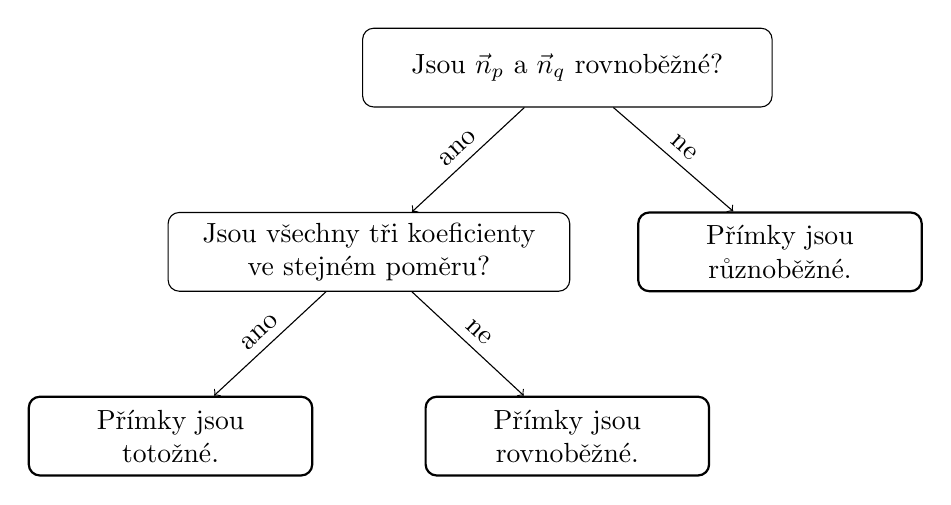
\begin{tikzpicture}[scale=0.9, every node/.style={align=center}]

        \node[draw, rounded corners, minimum width=5.2cm, minimum height=1cm]
            (start) at (0,0)
            {Jsou $\vec{n}_p$ a $\vec{n}_q$ rovnoběžné?};

        \node[draw, rounded corners, minimum width=5.1cm, minimum height=1cm]
            (coefficients) at (-2.8,-2.6)
            {Jsou všechny tři koeficienty\\ve stejném poměru?};

        \node[draw, rounded corners, minimum width=3.6cm, minimum height=1cm, thick]
            (intersecting) at (3,-2.6)
            {Přímky jsou\\různoběžné.};

        \node[draw, rounded corners, minimum width=3.6cm, minimum height=1cm, thick]
            (coincident) at (-5.6,-5.2)
            {Přímky jsou\\totožné.};

        \node[draw, rounded corners, minimum width=3.6cm, minimum height=1cm, thick]
            (parallel) at (0,-5.2)
            {Přímky jsou\\rovnoběžné.};

        \draw[->] (start) -- (coefficients)
            node[midway, above, sloped] {ano};
        \draw[->] (start) -- (intersecting)
            node[midway, above, sloped] {ne};
        \draw[->] (coefficients) -- (coincident)
            node[midway, above, sloped] {ano};
        \draw[->] (coefficients) -- (parallel)
            node[midway, above, sloped] {ne};

    \end{tikzpicture}
    \caption{Postup při určování vzájemné polohy přímek zadaných
    obecnými rovnicemi.}
    \label{fig:Relative_position_general_lines_decision}
\end{figure}

\paragraph{Rovnoběžné přímky}
\label{subsubsec:Parallel_general_lines}

Jsou-li normálové vektory dvou přímek rovnoběžné, mají přímky stejný
směr. Nejsou-li zároveň všechny tři koeficienty jejich obecných rovnic
ve stejném poměru, jde o dvě různé rovnoběžné přímky.

\begin{example}\label{exa:Parallel_general_lines}
    Určete vzájemnou polohu přímek $p:2x-3y+1=0$ a $q:-4x+6y+5=0$.
    
    Normálové vektory jsou
    \[
        \vec{n}_p=(2;-3),
        \qquad
        \vec{n}_q=(-4;6).
    \]
    Platí
    \[
        \vec{n}_q=-2\vec{n}_p,
    \]
    takže přímky mají stejný směr.

    Kdyby byly přímky totožné, musel by být stejným číslem $-2$
    vynásoben také absolutní člen. Platilo by tedy
    \[
        c_q=-2\cdot1=-2.
    \]
    Ve skutečnosti je však $c_q=5$. Všechny tři koeficienty proto
    nejsou ve stejném poměru a přímky jsou rovnoběžné:
    \[
        p\parallel q.
    \]
\end{example}

\begin{example}\label{exa:Parallel_general_line_through_point}
    Určete obecnou rovnici přímky $q$, která je rovnoběžná s přímkou $p:2x - 3y + 1 = 0$ a prochází bodem $K[-2;3]$.

    Rovnoběžná přímka může mít stejný normálový vektor
    \[
        \vec{n}_q=(2;-3).
    \]
    Její rovnice proto má tvar
    \[
        2x-3y+c=0.
    \]

    Dosadíme bod $K[-2;3]$:
    \begin{align*}
        2\cdot(-2)-3\cdot3+c&=0,\\
        -4-9+c&=0,\\
        c&=13.
    \end{align*}

    Hledaná přímka má rovnici
    \[
        q:2x-3y+13=0.
    \]
\end{example}

\paragraph{Různoběžné přímky a jejich průsečík}
\label{subsubsec:Intersecting_general_lines}

Nejsou-li normálové vektory dvou přímek rovnoběžné, mají přímky různé
směry a v rovině se protínají právě v jednom bodě. Souřadnice průsečíku
musí splňovat obě obecné rovnice současně, a proto je získáme řešením
soustavy těchto rovnic.

\begin{example}\label{exa:Intersecting_general_lines}
    Určete vzájemnou polohu přímek $p:2x+y-1=0$ a $q:x-y-2=0$.
    Jsou-li přímky různoběžné, určete jejich průsečík.

    Normálové vektory jsou
    \[
        \vec{n}_p=(2;1),
        \qquad
        \vec{n}_q=(1;-1).
    \]
    Tyto vektory nejsou rovnoběžné, protože neexistuje číslo $k$, pro
    které by platilo
    \[
        (1;-1)=k(2;1).
    \]
    Přímky jsou tedy různoběžné.

    Průsečík získáme řešením soustavy
    \begin{align*}
        2x+y-1&=0,\\
        x-y-2&=0.
    \end{align*}
    Po úpravě dostáváme
    \begin{align*}
        2x+y&=1,\\
        x-y&=2.
    \end{align*}

    Sečtením rovnic získáme
    \begin{align*}
        3x&=3,\\
        x&=1.
    \end{align*}
    Dosazením do druhé rovnice dostáváme
    \begin{align*}
        1-y&=2,\\
        y&=-1.
    \end{align*}

    Přímky se protínají v bodě
    \[
        P[1;-1],
    \]
    a proto
    \[
        p\cap q=\{P[1;-1]\}.
    \]
\end{example}

\paragraph{Totožné přímky}
\label{subsubsec:Coincident_general_lines}

Jsou-li všechny tři koeficienty jedné obecné rovnice stejným
nenulovým násobkem koeficientů druhé rovnice, popisují obě rovnice
tutéž množinu bodů. Přímky jsou proto totožné.

\begin{example}\label{exa:Coincident_general_lines}
    Určete vzájemnou polohu přímek $p:2x-3y+1=0$ a $q:-4x+6y-2=0$.

    Pro vektory platí
    \[
        (2;-3) = -\frac{1}{2}(-4;6)
    \]
    Z toho je zřejmé, že přímky jsou buď rovnoběžné anebo totožné.
    Zjistíme, zdali bod z přímky $p$ náleží přímce $q$. Najdemte tedy bod ležící na přímce $p$,
    tak že dosadíme jednu libovolnou souřadnici, např $x = -2$ a druhou dopočítáme. 

    \begin{align*}
        2 \cdot (-2) - 3y + 1 &= 0, \\
        -4 -3y +1 &= 0, \\
        -3y &= 3, \\
        y &= -1.
    \end{align*}

    Bod ležící na přímce $p$ je tedy $P[-2;-1]$. A ověříme zdali tento bod leží i na přímce $q$.

    \begin{align*}
        -4 \cdot (-2) + 6 \cdot (-1) - 2 &= 0, \\
        8 - 6 - 2 &= 0, \\
        0 &= 0.
    \end{align*}

    Protože bod $P[-2;-1]$ náleží oběma přímkám a zároveň jejich normálové vektory jsou rovnoběžné,
    pak jsou přímky totožné.

    Další způsob řešení je využítím toho, že pro koeficienty platí
    \[
        (-4;6;-2)=-2(2;-3;1).
    \]
    Druhá rovnice tedy vznikla vynásobením první rovnice číslem $-2$.
    Obě rovnice mají stejnou množinu řešení, a proto jsou přímky
    totožné:
    \[
        p=q.
    \]
    Jejich průnikem je celá přímka:
    \[
        p\cap q=p=q.
    \]
\end{example}

\paragraph{Kolmé přímky}
\label{subsubsec:Perpendicular_general_lines}

Dvě přímky jsou kolmé právě tehdy, když jsou kolmé jejich směrové
vektory. Protože pootočením obou vektorů o $90^\circ$ se velikost úhlu
mezi nimi nezmění, můžeme kolmost ověřovat také pomocí normálových
vektorů.

Pro přímky
\[
    p:a_1x+b_1y+c_1=0
\]
a
\[
    q:a_2x+b_2y+c_2=0
\]
platí
\begin{equation}\label{eq:Perpendicular_general_lines}
    p\perp q
    \quad\Longleftrightarrow\quad
    a_1a_2+b_1b_2=0.
\end{equation}

\begin{example}\label{exa:Perpendicular_general_lines}
    Určete vzájemnou polohu přímek
    \[
        p:x+2y-5=0
    \]
    a
    \[
        q:2x-y-5=0.
    \]

    Normálové vektory jsou
    \[
        \vec{n}_p=(1;2),
        \qquad
        \vec{n}_q=(2;-1).
    \]
    Jejich skalární součin je
    \[
        \vec{n}_p\cdot\vec{n}_q
        =
        1\cdot2+2\cdot(-1)
        =
        0.
    \]
    Přímky jsou proto kolmé:
    \[
        p\perp q.
    \]

    Jejich průsečík získáme řešením soustavy
    \begin{align*}
        x+2y&=5,\\
        2x-y&=5.
    \end{align*}
    Z druhé rovnice vyjádříme
    \[
        y=2x-5
    \]
    a dosadíme do první:
    \begin{align*}
        x+2(2x-5)&=5,\\
        5x-10&=5,\\
        x&=3.
    \end{align*}
    Potom
    \[
        y=2\cdot3-5=1.
    \]
    Kolmé přímky se protínají v bodě
    \[
        P[3;1].
    \]
\end{example}

\begin{example}\label{exa:Perpendicular_general_line_through_point}
    Určete obecnou rovnici přímky $q$, která je kolmá k přímce $p:2x-3y+1=0$ a prochází bodem $K[-2;3]$.
    
    Normálový vektor přímky $p$ je
    \[
        \vec{n}_p=(2;-3).
    \]
    Směrový vektor přímky $p$ můžeme zvolit například
    \[
        \vec{u}_p=(3;2).
    \]

    Hledaná přímka $q$ má být k přímce $p$ kolmá. Její normálový vektor
    proto může být rovnoběžný se směrovým vektorem přímky $p$. Zvolíme
    \[
        \vec{n}_q=(3;2).
    \]

    Rovnice hledané přímky má tvar
    \[
        3x+2y+c=0.
    \]
    Dosadíme bod $K[-2;3]$:
    \begin{align*}
        3\cdot(-2)+2\cdot3+c&=0,\\
        -6+6+c&=0,\\
        c&=0.
    \end{align*}

    Hledaná kolmice má rovnici
    \[
        q:3x+2y=0.
    \]
\end{example}

\begin{example}\label{exa:Central_symmetry_line}
    Je dána přímka
    \[
        p:2x-y+1=0.
    \]
    Určete rovnici přímky $p'$, která je obrazem přímky $p$ ve
    středové souměrnosti se středem
    \[
        S[-2;1].
    \]

    Přímku $p'$ můžeme určit pomocí obrazů dvou různých bodů přímky
    $p$. Pro obraz libovolného bodu $X$ ve středové souměrnosti se
    středem $S$ platí
    \[
        X'=S+(S-X)=2S-X.
    \]

    Nejprve tedy na přímce $p$ zvolíme dva různé body, určíme jejich
    obrazy a následně sestavíme rovnici přímky procházející těmito
    obrazy.

    Zvolíme nejprve bod s první souřadnicí $x=0$. Dosadíme do rovnice
    přímky $p$:
    \begin{align*}
        2\cdot0-y+1&=0,\\
        -y+1&=0,\\
        y&=1.
    \end{align*}

    Na přímce $p$ tedy leží bod
    \[
        A[0;1].
    \]

    Jako druhý bod zvolíme bod s první souřadnicí $x=1$:
    \begin{align*}
        2\cdot1-y+1&=0,\\
        3-y&=0,\\
        y&=3.
    \end{align*}

    Druhým bodem přímky $p$ je
    \[
        B[1;3].
    \]

    Nyní určíme obraz bodu $A$ ve středové souměrnosti se středem
    $S[-2;1]$:
    \begin{align*}
        A'
        &=
        S+(S-A)\\
        &=
        [-2;1]+\bigl([-2;1]-[0;1]\bigr)\\
        &=
        [-2;1]+(-2;0)\\
        &=
        [-4;1].
    \end{align*}

    Obdobně určíme obraz bodu $B$:
    \begin{align*}
        B'
        &=
        S+(S-B)\\
        &=
        [-2;1]+\bigl([-2;1]-[1;3]\bigr)\\
        &=
        [-2;1]+(-3;-2)\\
        &=
        [-5;-1].
    \end{align*}

    Obrazem přímky $p$ je přímka $p'$, která prochází body
    \[
        A'[-4;1]
        \qquad\text{a}\qquad
        B'[-5;-1].
    \]

    Její směrový vektor můžeme určit jako
    \[
        \overrightarrow{A'B'}
        =
        (-5-(-4);-1-1)
        =
        (-1;-2).
    \]

    K tomuto směrovému vektoru zvolíme normálový vektor
    \[
        \vec{n}_{p'}=(2;-1),
    \]
    protože
    \[
        (-1;-2)\cdot(2;-1)
        =
        -2+2
        =
        0.
    \]

    Obecná rovnice přímky $p'$ má tedy tvar
    \[
        2x-y+c=0.
    \]

    Dosadíme například bod $A'[-4;1]$:
    \begin{align*}
        2\cdot(-4)-1+c&=0,\\
        -8-1+c&=0,\\
        c&=9.
    \end{align*}

    Hledaná přímka má rovnici
    \[
        p':2x-y+9=0.
    \]

    Přímky $p$ a $p'$ mají stejné normálové vektory, a jsou proto
    rovnoběžné. To odpovídá vlastnosti středové souměrnosti: obrazem
    přímky, která neprochází středem souměrnosti, je přímka s ní
    rovnoběžná.

    \begin{figure}[H]
        \centering
        \begin{tikzpicture}[scale=0.9]

            % Přímky
            \draw[thin, <->]
                (-1.5,-2) -- (2.5,6)
                node[above right] {$p$};

            \draw[thin, <->]
                (-5.5,-2) -- (-1.5,6)
                node[above right] {$p'$};

            % Body
            \coordinate (A) at (0,1);
            \coordinate (B) at (1,3);
            \coordinate (S) at (-2,1);
            \coordinate (Ap) at (-4,1);
            \coordinate (Bp) at (-5,-1);

            \fill (A) circle (2.5pt)
                node[below right] {$A$};
            \fill (B) circle (2.5pt)
                node[below right] {$B$};
            \fill (S) circle (2.5pt)
                node[above right] {$S$};
            \fill (Ap) circle (2.5pt)
                node[above left] {$A'$};
            \fill (Bp) circle (2.5pt)
                node[below left] {$B'$};

            % Spojnice bodů se středem
            \draw[vector] (A) -- (S);
            \draw[vector] (S) -- (Ap);

            \draw[vector] (B) -- (S);
            \draw[vector] (S) -- (Bp);

        \end{tikzpicture}
        \caption{Přímka $p'$ je obrazem přímky $p$ ve středové
        souměrnosti se středem $S$.}
        \label{fig:Central_symmetry_line}
    \end{figure}
\end{example}
\subsubsection{Vzájemná poloha přímek ve směrnicovém tvaru}
\label{subsubsec:Relative_position_slope_intercept_lines}

Ve směrnicovém tvaru je směr přímky určen přímo její směrnicí.
Vzájemnou polohu dvou nesvislých přímek proto můžeme určit porovnáním
jejich směrnic a úseků na ose $y$.

Uvažujme dvě přímky
\begin{align*}
    p &: y=k_1x+q_1,\\
    q &: y=k_2x+q_2.
\end{align*}

Jejich směr určují směrnice $k_1$ a $k_2$.

Jestliže
\[
    k_1\neq k_2,
\]
mají přímky různé směry, a proto jsou různoběžné. Jejich průsečík
získáme řešením rovnice
\[
    k_1x+q_1=k_2x+q_2.
\]

Odtud
\begin{equation}\label{eq:Slope_intercept_intersection_x}
    x_P=\frac{q_2-q_1}{k_1-k_2}.
\end{equation}

Druhou souřadnici průsečíku získáme dosazením hodnoty $x_P$ do rovnice
jedné z přímek.

Jestliže
\[
    k_1=k_2,
\]
mají přímky stejný směr. Potom rozlišujeme dva případy:
\begin{itemize}
    \item je-li $q_1\neq q_2$, jsou přímky rovnoběžné;
    \item je-li $q_1=q_2$, jsou přímky totožné.
\end{itemize}

Celý postup můžeme shrnout následovně:
\[
\begin{array}{c|c}
    \text{Podmínka}
    &
    \text{Vzájemná poloha přímek}
    \\
    \hline
    k_1\neq k_2
    &
    \text{přímky jsou různoběžné}
    \\[1mm]
    k_1=k_2,\ q_1\neq q_2
    &
    \text{přímky jsou rovnoběžné}
    \\[1mm]
    k_1=k_2,\ q_1=q_2
    &
    \text{přímky jsou totožné}
\end{array}
\]

\begin{example}\label{exa:Relative_position_slope_intercept_lines}
    Určete vzájemnou polohu přímek $p:y=2x-3$ a $q:y=-x+3$.

    Jejich směrnice jsou
    \[
        k_p=2,
        \qquad
        k_q=-1.
    \]
    Protože
    \[
        k_p\neq k_q,
    \]
    jsou přímky různoběžné.

    Souřadnici $x$ průsečíku získáme z rovnosti
    \begin{align*}
        2x-3&=-x+3,\\
        3x&=6,\\
        x&=2.
    \end{align*}

    Dosadíme do první rovnice:
    \[
        y=2\cdot2-3=1.
    \]

    Přímky se protínají v bodě
    \[
        P[2;1],
    \]
    a proto
    \[
        p\cap q=\{P[2;1]\}.
    \]
\end{example}

\paragraph{Kolmé přímky ve směrnicovém tvaru}
\label{subsubsec:Perpendicular_slope_intercept_lines}

Uvažujme dvě nesvislé přímky se směrnicemi $k_1$ a $k_2$. Jako jejich
směrové vektory můžeme podle vztahu
\eqref{eq:Direction_vector_from_slope} zvolit
\[
    \vec{u}_1=(1;k_1),
    \qquad
    \vec{u}_2=(1;k_2).
\]

Přímky jsou kolmé právě tehdy, když jsou kolmé jejich směrové vektory.
Jejich skalární součin proto musí být roven nule:
\begin{align*}
    \vec{u}_1\cdot\vec{u}_2
    &=
    (1;k_1)\cdot(1;k_2),\\
    0
    &=
    1+k_1k_2.
\end{align*}

Odtud dostáváme podmínku
\begin{equation}\label{eq:Perpendicular_slopes}
    k_1k_2=-1.
\end{equation}

Je-li $k_1\neq0$, můžeme směrnici kolmé přímky vyjádřit jako
\begin{equation}\label{eq:Perpendicular_slope}
    k_2=-\frac{1}{k_1}.
\end{equation}

Směrnice navzájem kolmých nesvislých přímek jsou tedy čísla
s opačnými znaménky a převrácenými absolutními hodnotami.

\begin{remark}\label{rem:Vertical_horizontal_perpendicular_lines}
    Vztah \eqref{eq:Perpendicular_slopes} lze použít pouze tehdy,
    když mají obě přímky definovanou směrnici. Svislá přímka nemá
    směrnici a je kolmá ke každé vodorovné přímce tvaru
    \[
        y=q.
    \]
\end{remark}

\begin{example}\label{exa:Perpendicular_line_slope_intercept}
    Určete směrnicový tvar přímky $q$, která prochází bodem $A[2;1]$ a je kolmá k přímce $p:y=2x+1$.

    Směrnice přímky $p$ je
    \[
        k_p=2.
    \]

    Směrnice kolmé přímky je
    \[
        k_q=-\frac{1}{2}.
    \]

    Použijeme bodově-směrnicový tvar:
    \begin{align*}
        y-1
        &=
        -\frac{1}{2}(x-2),\\
        y-1
        &=
        -\frac{1}{2}x+1,\\
        y
        &=
        -\frac{1}{2}x+2.
    \end{align*}

    Hledaná přímka má rovnici
    \[
        q:y=-\frac{1}{2}x+2.
    \]

    Kolmost můžeme ověřit součinem směrnic:
    \[
        2\cdot\left(-\frac{1}{2}\right)=-1.
    \]
\end{example}
\subsubsection{Vzájemná poloha přímek zadaných v různých tvarech}
\label{subsubsec:Relative_position_mixed_line_forms}

V předchozích částech byly obě přímky zadány stejným způsobem.
V úlohách však mohou být jednotlivé přímky zadány také různými tvary.

Jedna přímka může být například zadána parametricky a druhá obecnou
rovnicí. V takovém případě můžeme jednu z nich převést do stejného
tvaru jako druhou pomocí postupů uvedených v podsekci
\ref{subsec:Conversions_between_line_forms}. Úplný převod však není
vždy nutný. Často postačí z obou zápisů určit údaj popisující směr
přímky a tyto údaje porovnat.

Při určování vzájemné polohy budeme používat především následující
informace:

\begingroup
\renewcommand{\arraystretch}{1.6}
\[
\begin{array}{c|c|c}
    \text{způsob zadání}
    &
    \text{údaj určující směr}
    &
    \text{další užitečný údaj}
    \\
    \hline
    \text{parametrické vyjádření}
    &
    \vec{u}=(u_x;u_y)
    &
    A[x_A;y_A]
    \\[1mm]
    \text{obecná rovnice}
    &
    \vec{n}=(a;b)
    &
    \vec{u}=(-b;a)
    \\[1mm]
    \text{směrnicový tvar}
    &
    k
    &
    \vec{u}=(1;k),\quad Q[0;q]
\end{array}
\]
\endgroup

Při řešení tedy můžeme postupovat dvěma způsoby:

\begin{enumerate}
    \item jednu přímku převedeme do stejného tvaru jako druhou
    a použijeme již známý postup;
    \item bez úplného převodu porovnáme směrové nebo normálové vektory,
    případně směrnice, a průsečík určíme přímým dosazením jednoho
    zápisu do druhého.
\end{enumerate}

Druhý postup bývá zpravidla kratší, protože využívá pouze ty údaje,
které jsou pro určení vzájemné polohy skutečně potřebné.


\paragraph{Parametrické vyjádření a obecná rovnice}

Uvažujme přímku $p$ zadanou parametricky
\begin{equation}\label{eq:Mixed_parametric_general_p}
    \begin{aligned}
        p:\quad x&=x_A+t u_x,\\
                 y&=y_A+t u_y,
                 \qquad t\in\mathbb{R},
    \end{aligned}
\end{equation}
a přímku $q$ zadanou obecnou rovnicí
\begin{equation}\label{eq:Mixed_parametric_general_q}
    q:\quad ax+by+c=0.
\end{equation}

Směr přímky $p$ je určen směrovým vektorem
\[
    \vec{u}_p=(u_x;u_y),
\]
zatímco přímka $q$ má normálový vektor
\[
    \vec{n}_q=(a;b).
\]

Přímky mají stejný směr právě tehdy, když je směrový vektor přímky
$p$ kolmý k normálovému vektoru přímky $q$. Tuto podmínku můžeme
zapsat jako
\begin{equation}\label{eq:Mixed_parametric_general_parallel_condition}
    \vec{u}_p\cdot\vec{n}_q
    =
    au_x+bu_y
    =
    0.
\end{equation}

Jestliže
\[
    au_x+bu_y\neq0,
\]
přímky nemají stejný směr, a jsou proto různoběžné.

Jestliže naopak
\[
    au_x+bu_y=0,
\]
mají přímky stejný směr. Potom musíme ještě rozhodnout, zda jsou
rovnoběžné, nebo totožné. Stačí ověřit, zda zvolený bod
$A[x_A;y_A]$ parametricky zadané přímky leží také na přímce $q$:

\[
\begin{array}{c|c}
    ax_A+by_A+c\neq0
    &
    p\parallel q
    \\[1mm]
    ax_A+by_A+c=0
    &
    p=q
\end{array}
\]

Průsečík různoběžných přímek můžeme určit bez převodu celé rovnice.
Parametrické rovnice přímky $p$ dosadíme přímo do obecné rovnice
přímky $q$:
\begin{align*}
    a(x_A+t u_x)+b(y_A+t u_y)+c&=0,\\
    ax_A+at u_x+by_A+bt u_y+c&=0,\\
    t(au_x+bu_y)+ax_A+by_A+c&=0.
\end{align*}

Je-li $au_x+bu_y\neq0$, získáme jedinou hodnotu parametru
\begin{equation}\label{eq:Mixed_parametric_general_intersection_parameter}
    t
    =
    -\frac{ax_A+by_A+c}{au_x+bu_y}.
\end{equation}
Po jejím dosazení do parametrického vyjádření přímky $p$ získáme
souřadnice průsečíku.

\begin{remark}\label{rem:Mixed_parametric_general_equation_meaning}
    Rovnice vzniklá dosazením parametrického vyjádření do obecné
    rovnice může mít tři různé podoby:

    \begin{itemize}
        \item má právě jedno řešení pro $t$; přímky jsou různoběžné;
        \item vznikne nepravdivý výrok, například $5=0$; přímky jsou
        rovnoběžné a různé;
        \item vznikne pravdivý výrok, například $0=0$; každý bod
        parametricky zadané přímky splňuje obecnou rovnici, a přímky
        jsou proto totožné.
    \end{itemize}
\end{remark}

Kolmost lze určit také přímo. Přímka $q$ je kolmá ke svému normálovému
vektoru $\vec{n}_q$. Proto platí
\[
    p\perp q
\]
právě tehdy, když jsou vektory $\vec{u}_p$ a $\vec{n}_q$ rovnoběžné.

\begin{example}\label{exa:Mixed_parametric_general_intersection}
    Určete vzájemnou polohu přímek
    \[
        \begin{aligned}
            p:\quad x&=1+2t,\\
                     y&=2-t,
                     \qquad t\in\mathbb{R},
        \end{aligned}
    \]
    a
    \[
        q:\quad x+y-4=0.
    \]
    Jsou-li přímky různoběžné, určete jejich průsečík.

    Směrový vektor přímky $p$ a normálový vektor přímky $q$ jsou
    \[
        \vec{u}_p=(2;-1),
        \qquad
        \vec{n}_q=(1;1).
    \]

    Vypočítáme jejich skalární součin:
    \[
        \vec{u}_p\cdot\vec{n}_q
        =
        (2;-1)\cdot(1;1)
        =
        2-1
        =
        1.
    \]

    Skalární součin není roven nule, takže směrový vektor přímky $p$
    není kolmý k normálovému vektoru přímky $q$. Přímky tedy nemají
    stejný směr a jsou různoběžné.

    Průsečík určíme dosazením parametrických rovnic přímky $p$ do
    obecné rovnice přímky $q$:
    \begin{align*}
        (1+2t)+(2-t)-4&=0,\\
        1+2t+2-t-4&=0,\\
        t-1&=0,\\
        t&=1.
    \end{align*}

    Hodnotu $t=1$ dosadíme do parametrického vyjádření:
    \begin{align*}
        x&=1+2\cdot1=3,\\
        y&=2-1=1.
    \end{align*}

    Průsečíkem přímek je bod
    \[
        P[3;1].
    \]

    Výsledek ověříme dosazením do obecné rovnice:
    \[
        3+1-4=0.
    \]

    Platí tedy
    \[
        p\cap q=\{P[3;1]\}.
    \]
\end{example}


\paragraph{Parametrické vyjádření a směrnicový tvar}

Uvažujme přímku $p$ zadanou parametricky
\begin{equation}\label{eq:Mixed_parametric_slope_p}
    \begin{aligned}
        p:\quad x&=x_A+t u_x,\\
                 y&=y_A+t u_y,
                 \qquad t\in\mathbb{R},
    \end{aligned}
\end{equation}
a přímku $q$ ve směrnicovém tvaru
\begin{equation}\label{eq:Mixed_parametric_slope_q}
    q:\quad y=kx+q_0.
\end{equation}

Směrový vektor přímky $p$ je
\[
    \vec{u}_p=(u_x;u_y),
\]
zatímco jako směrový vektor přímky $q$ můžeme zvolit
\[
    \vec{u}_q=(1;k).
\]

Přímky mají stejný směr právě tehdy, když jsou jejich směrové vektory
rovnoběžné. Jestliže $u_x\neq0$, můžeme tuto podmínku zapsat jako
\[
    \frac{u_y}{u_x}=k.
\]

Podmínku lze zapsat také bez dělení:
\begin{equation}\label{eq:Mixed_parametric_slope_parallel_condition}
    u_y-ku_x=0.
\end{equation}

Tento zápis je výhodný také při rozlišování svislé přímky. Je-li
$u_x=0$, potom musí platit $u_y\neq0$, a proto
\[
    u_y-ku_x=u_y\neq0.
\]
Svislá parametricky zadaná přímka tedy nemůže být rovnoběžná s přímkou
ve směrnicovém tvaru a vždy ji protíná.

Jestliže
\[
    u_y-ku_x\neq0,
\]
jsou přímky různoběžné.

Jestliže
\[
    u_y-ku_x=0,
\]
mají přímky stejný směr. Jejich totožnost ověříme dosazením bodu
$A[x_A;y_A]$ do směrnicové rovnice:
\[
\begin{array}{c|c}
    y_A\neq kx_A+q_0
    &
    p\parallel q
    \\[1mm]
    y_A=kx_A+q_0
    &
    p=q
\end{array}
\]

Průsečík různoběžných přímek určíme dosazením parametrických rovnic
do směrnicového tvaru:
\begin{align*}
    y_A+t u_y
    &=
    k(x_A+t u_x)+q_0,\\
    y_A+t u_y
    &=
    kx_A+kt u_x+q_0,\\
    t(u_y-ku_x)
    &=
    kx_A+q_0-y_A.
\end{align*}

Je-li $u_y-ku_x\neq0$, dostáváme
\begin{equation}\label{eq:Mixed_parametric_slope_intersection_parameter}
    t
    =
    \frac{kx_A+q_0-y_A}{u_y-ku_x}.
\end{equation}

Kolmost přímek můžeme určit pomocí skalárního součinu jejich směrových
vektorů:
\[
    \vec{u}_p\cdot\vec{u}_q
    =
    (u_x;u_y)\cdot(1;k)
    =
    u_x+ku_y.
\]
Proto platí
\begin{equation}\label{eq:Mixed_parametric_slope_perpendicular_condition}
    p\perp q
    \quad\Longleftrightarrow\quad
    u_x+ku_y=0.
\end{equation}

\begin{example}\label{exa:Mixed_parametric_slope_parallel_coincident}
    Je dána parametricky zadaná přímka
    \[
        \begin{aligned}
            p:\quad x&=1+2t,\\
                     y&=2+t,
                     \qquad t\in\mathbb{R},
        \end{aligned}
    \]
    a přímky ve směrnicovém tvaru
    \[
        q:\quad y=\frac12x+3,
    \]
    \[
        r:\quad y=\frac12x+\frac32.
    \]

    Určete vzájemnou polohu dvojic přímek $p$, $q$ a přímek $p$, $r$.

    Směrový vektor přímky $p$ je
    \[
        \vec{u}_p=(2;1),
    \]
    a její směrnice je proto
    \[
        k_p=\frac12.
    \]

    Přímky $q$ i $r$ mají rovněž směrnici
    \[
        k_q=k_r=\frac12.
    \]
    Všechny tři přímky tedy mají stejný směr.

    Nejprve ověříme, zda bod $A[1;2]$ přímky $p$ leží na přímce $q$:
    \[
        \frac12\cdot1+3
        =
        \frac72
        \neq
        2.
    \]
    Bod $A$ na přímce $q$ neleží. Přímky $p$ a $q$ mají stejný směr,
    ale nejsou totožné, a proto
    \[
        p\parallel q.
    \]

    Nyní dosadíme bod $A[1;2]$ do rovnice přímky $r$:
    \[
        \frac12\cdot1+\frac32
        =
        2.
    \]
    Bod $A$ na přímce $r$ leží. Přímky $p$ a $r$ mají stejný směr
    a společný bod, a proto jsou totožné:
    \[
        p=r.
    \]
\end{example}


\paragraph{Obecná rovnice a směrnicový tvar}

Uvažujme přímku $p$ zadanou obecnou rovnicí
\begin{equation}\label{eq:Mixed_general_slope_p}
    p:\quad ax+by+c=0
\end{equation}
a přímku $q$ ve směrnicovém tvaru
\begin{equation}\label{eq:Mixed_general_slope_q}
    q:\quad y=kx+q_0.
\end{equation}

Normálový vektor přímky $p$ je
\[
    \vec{n}_p=(a;b),
\]
zatímco směrový vektor přímky $q$ můžeme zvolit jako
\[
    \vec{u}_q=(1;k).
\]

Přímky mají stejný směr právě tehdy, když je směrový vektor přímky
$q$ kolmý k normálovému vektoru přímky $p$:
\[
    \vec{n}_p\cdot\vec{u}_q
    =
    (a;b)\cdot(1;k)
    =
    a+bk.
\]

Podmínka stejného směru tedy je
\begin{equation}\label{eq:Mixed_general_slope_parallel_condition}
    a+bk=0.
\end{equation}

Je-li $b=0$, obecná rovnice popisuje svislou přímku. Protože potom
$a\neq0$, platí
\[
    a+bk=a\neq0.
\]
Svislá přímka se tedy s každou přímkou ve směrnicovém tvaru protíná.

Jestliže
\[
    a+bk\neq0,
\]
jsou přímky různoběžné.

Jestliže
\[
    a+bk=0,
\]
mají přímky stejný směr. K rozlišení rovnoběžnosti a totožnosti
použijeme například bod
\[
    Q[0;q_0],
\]
který leží na přímce $q$. Po dosazení do obecné rovnice přímky $p$
dostáváme
\[
\begin{array}{c|c}
    bq_0+c\neq0
    &
    p\parallel q
    \\[1mm]
    bq_0+c=0
    &
    p=q
\end{array}
\]

Průsečík různoběžných přímek získáme dosazením směrnicové rovnice do
obecné rovnice:
\begin{align*}
    ax+b(kx+q_0)+c&=0,\\
    ax+bkx+bq_0+c&=0,\\
    (a+bk)x+bq_0+c&=0.
\end{align*}

Je-li $a+bk\neq0$, dostáváme
\begin{equation}\label{eq:Mixed_general_slope_intersection_x}
    x
    =
    -\frac{bq_0+c}{a+bk}.
\end{equation}
Druhou souřadnici průsečíku určíme ze vztahu
\[
    y=kx+q_0.
\]

Kolmost můžeme určit porovnáním směrových vektorů. Jako směrový vektor
přímky $p$ můžeme zvolit
\[
    \vec{u}_p=(-b;a),
\]
zatímco pro přímku $q$ máme
\[
    \vec{u}_q=(1;k).
\]
Přímky jsou kolmé právě tehdy, když
\[
    \vec{u}_p\cdot\vec{u}_q
    =
    (-b;a)\cdot(1;k)
    =
    -b+ak
    =
    0.
\]
Tedy
\begin{equation}\label{eq:Mixed_general_slope_perpendicular_condition}
    p\perp q
    \quad\Longleftrightarrow\quad
    ak-b=0.
\end{equation}

\begin{example}\label{exa:Mixed_general_slope_perpendicular}
    Určete vzájemnou polohu přímek
    \[
        p:\quad x+2y-5=0
    \]
    a
    \[
        q:\quad y=2x.
    \]
    Jsou-li přímky různoběžné, určete jejich průsečík.

    Pro obecnou rovnici přímky $p$ platí
    \[
        a=1,
        \qquad
        b=2,
        \qquad
        c=-5.
    \]
    Směrnice přímky $q$ je
    \[
        k=2,
        \qquad
        q_0=0.
    \]

    Nejprve ověříme podmínku stejného směru:
    \[
        a+bk
        =
        1+2\cdot2
        =
        5.
    \]
    Výsledek není roven nule, takže přímky nemají stejný směr a jsou
    různoběžné.

    Současně platí
    \[
        ak-b
        =
        1\cdot2-2
        =
        0.
    \]
    Přímky jsou tedy kolmé.

    Průsečík určíme dosazením rovnice $y=2x$ do obecné rovnice:
    \begin{align*}
        x+2(2x)-5&=0,\\
        x+4x-5&=0,\\
        5x&=5,\\
        x&=1.
    \end{align*}

    Druhou souřadnici získáme ze směrnicové rovnice:
    \[
        y=2\cdot1=2.
    \]

    Průsečíkem je bod
    \[
        P[1;2].
    \]

    Platí tedy
    \[
        p\perp q
        \qquad\text{a}\qquad
        p\cap q=\{P[1;2]\}.
    \]
\end{example}

\begin{example}\label{exa:Mixed_line_forms_summary}
    Jsou dány tři přímky, z nichž je každá zadaná jiným způsobem:
    \[
        \begin{aligned}
            p:\quad x&=t,\\
                     y&=2t,
                     \qquad t\in\mathbb{R},
        \end{aligned}
    \]
    \[
        q:\quad 2x-y+5=0,
    \]
    \[
        r:\quad y=-\frac12x+\frac52.
    \]

    Určete vzájemnou polohu každé dvojice přímek. U různoběžných
    přímek určete také jejich průsečík.

    \begin{enumerate}[label=\alph*)]
        \item Přímky $p$ a $q$,
        \item přímky $p$ a $r$,
        \item přímky $q$ a $r$.
    \end{enumerate}

    Nejprve z jednotlivých zápisů získáme údaje popisující směr
    přímek.

    Přímka $p$ má směrový vektor
    \[
        \vec{u}_p=(1;2).
    \]

    Přímka $q$ má normálový vektor
    \[
        \vec{n}_q=(2;-1),
    \]
    a proto jako její směrový vektor můžeme zvolit
    \[
        \vec{u}_q=(1;2).
    \]

    Přímka $r$ má směrnici
    \[
        k_r=-\frac12.
    \]
    Jako její směrový vektor můžeme zvolit
    \[
        \vec{u}_r=(2;-1).
    \]

    \begin{enumerate}[label=\alph*), leftmargin=2em]

        \item \textbf{Přímky $p$ a $q$}

        Směrové vektory přímek jsou totožné:
        \[
            \vec{u}_p=\vec{u}_q=(1;2).
        \]
        Přímky tedy mají stejný směr.

        Bod $A[0;0]$ leží na přímce $p$. Dosadíme jej do obecné rovnice
        přímky $q$:
        \[
            2\cdot0-0+5=5\neq0.
        \]
        Bod $A$ na přímce $q$ neleží, a proto jsou přímky rovnoběžné
        a různé:
        \[
            p\parallel q.
        \]

        \item \textbf{Přímky $p$ a $r$}

        Vypočítáme skalární součin jejich směrových vektorů:
        \[
            \vec{u}_p\cdot\vec{u}_r
            =
            (1;2)\cdot(2;-1)
            =
            2-2
            =
            0.
        \]
        Přímky jsou tedy kolmé, a proto různoběžné.

        Průsečík určíme dosazením parametrického vyjádření přímky $p$
        do směrnicové rovnice přímky $r$:
        \begin{align*}
            2t
            &=
            -\frac12t+\frac52,\\
            \frac52t
            &=
            \frac52,\\
            t&=1.
        \end{align*}

        Pro $t=1$ dostáváme
        \[
            P[1;2].
        \]

        Platí tedy
        \[
            p\perp r
            \qquad\text{a}\qquad
            p\cap r=\{P[1;2]\}.
        \]

        \item \textbf{Přímky $q$ a $r$}

        Přímka $q$ má směrový vektor
        \[
            \vec{u}_q=(1;2),
        \]
        zatímco přímka $r$ má směrový vektor
        \[
            \vec{u}_r=(2;-1).
        \]
        Jejich skalární součin je
        \[
            (1;2)\cdot(2;-1)=2-2=0.
        \]
        Přímky jsou tedy také kolmé.

        Průsečík určíme dosazením směrnicové rovnice přímky $r$ do
        obecné rovnice přímky $q$:
        \begin{align*}
            2x-\left(-\frac12x+\frac52\right)+5&=0,\\
            2x+\frac12x-\frac52+5&=0,\\
            \frac52x+\frac52&=0,\\
            x&=-1.
        \end{align*}

        Druhou souřadnici dopočítáme ze směrnicové rovnice:
        \[
            y
            =
            -\frac12(-1)+\frac52
            =
            \frac12+\frac52
            =
            3.
        \]

        Průsečíkem je bod
        \[
            Q[-1;3].
        \]

        Platí tedy
        \[
            q\perp r
            \qquad\text{a}\qquad
            q\cap r=\{Q[-1;3]\}.
        \]

    \end{enumerate}

    Výsledky můžeme shrnout:
    \[
    \begin{array}{c|c|c}
        \text{dvojice přímek}
        &
        \text{vzájemná poloha}
        &
        \text{průsečík}
        \\
        \hline
        p,\ q
        &
        \text{rovnoběžné}
        &
        \varnothing
        \\[1mm]
        p,\ r
        &
        \text{kolmé}
        &
        P[1;2]
        \\[1mm]
        q,\ r
        &
        \text{kolmé}
        &
        Q[-1;3]
    \end{array}
    \]
\end{example}

Při určování vzájemné polohy přímek zadaných různými způsoby tedy není
nutné vždy provádět úplný převod. Často stačí z každého zápisu získat
směrový nebo normálový vektor, případně směrnici, a průsečík určit
přímým dosazením. Volba postupu závisí na konkrétním zadání a na tom,
který zápis vede k nejjednoduššímu výpočtu.
